\documentclass{xduugthesis}
\usepackage[ruled,linesnumbered]{algorithm2e}
\renewcommand{\algorithmcfname}{算法}
\setmonofont{Courier New}
\usepackage{flowchart, listings, fontspec}
\usetikzlibrary{shapes.geometric, arrows}
\usepackage{subcaption}
\usepackage{paralist}
\usepackage[inline]{enumitem}
\xdusetup{
	style = {
		cjk-font=win,
		latin-font=tac,
		math-font=xits,
		subsec-zihao=-4,
		after-skip = {18pt,12pt,12pt,12pt,10pt,10pt},
		before-skip = {20pt,14pt,14pt,14pt,12pt,12pt},
	},
	info = {
		abstract = {abstract.txt},
		abstract* = {abstract-eng.txt},
		keywords = {合成孔径雷达;图像融合;MATLAB仿真},
		keywords* = {Synthetic ApertureRadar, Image Fusion, MATLAB Simulation},
		acknowledgements = {acknowledgements.txt},
		title = {合成孔径雷达图像融合软件的设计\\与实现},
		author = {author.txt},
		department = {计算机科学技术学院},
		class-id = {classid.txt},
		student-id = {student-id.txt},
		major = {软件工程},
		supervisor = {teacher.txt},
		bib-resource={thesis.bib}
	}
}
\begin{document}
\lstset{
	numbers=left,
	basicstyle=\fontsize{9}{11}\selectfont\ttfamily,
	numberstyle=\tiny,
	keywordstyle=\color{blue!70},
	commentstyle=\color{red!50!green!50!blue!50},
	frame=shadowbox,
	rulesepcolor=\color{red!20!green!20!blue!20}
}
\chapter{概述}
\section{研究背景和意义}
合成孔径雷达(Synthetic Aperture Radar, SAR)是一种利用雷达信号的相位和幅度信息来生成图像的技术。
它通过移动的雷达平台发射和接收信号,然后对这些信号进行处理,以产生高分辨率的图像。SAR技术在军事、地质勘
探、环境监测、农业和城市规划等多个领域有着广泛的应用。\par
在对遥感图像进行目标识别的情况下,使用者需要融合大量的图像。在融合过程中,使用不同的图像分解方法和加权融
合算法会影响融合结果的质量。为此,本毕设实现了一些图像融合算法,同时实现了对融合结果的量化评估。为更好评
估图像融合效果,本毕设实现了对一个目标点进行多角度成像的雷达仿真,从而获得仿真模拟数据。\par
在上述研究的基础上,本毕设实现了一个合成孔径雷达图像融合软件。该软件可以对进行合成孔径雷达的多角度成像仿
真,并融合多角度雷达成像,并对融合图像进行量化评估。该程序功能明了,使用方便。通过本程序,使用者可以进一
步了解对合成孔径雷达的成像过程,并更加方便地融合多角度雷达图像。\par
\section{研究内容}
本毕业设计的核心目标是解决三个关键问题:仿真生成多角度合成孔径雷达图像,图像融合算法的实现,以及编写便于使
用的合成孔径雷达图像融合软件。\par

在仿真生成多角度雷达图像方面,本毕设充分利用了MATLAB这一强大的模拟仿真平台。首先,通过构建模拟地形并合理
放置目标点,为雷达成像提供了一个真实的测试环境。随后,模拟雷达对地形上目标点进行多角度扫描,模拟实际的合成
孔径雷达成像过程,生成了多角度成像的仿真模拟数据,这些数据不仅为图像融合提供了必要的输入,也为算法的验证和
优化提供了实验基础。\par

在图像融合算法的实现方面,本毕设深入学习了现有的经典图像分解和融合技术。通过对这些算法的深入理解和应
用,本毕设根据合成孔径雷达图像的信息特征,实现了一些图像融合方法,以提升雷达图像的信息量。此外,为了更全面
地评估融合效果,本毕设还实现了对融合图像的量化分析,能够对融合后图像的多种量化指标进行测量和分析。\par

在合成孔径雷达图像融合软件的开发过程中,本毕设整合了仿真生成多角度雷达图像和图像融合算法的研究与实现,同时
加入了用户输入多角度雷达图像功能,并提供了清晰的命令行界面和简洁的操作流程。最终,本毕设实现了一个功能完备、
操作简便、用户友好的合成孔径雷达图像融合软件。
\section{论文结构}
本论文共分为五章,具体结构如下所述。\par
第一章是概述。作为论文的开篇,首先明确了本毕业设计的研究目的和意义,提出了需要解决的关键问题。接着,本章概述
了整个毕业设计的研究架构和研究方法,为读者提供了一个清晰的研究路线图。\par
第二章是相关技术背景。在这一章节中,本毕设深入探讨了与研究主题相关的技术背景。首先,对合成孔径雷达的基本原理
和成像技术进行了介绍,包括该种雷达的工作原理、成像模式,波长介绍和模拟软件一览。随后,本章详细阐述了本毕设所
采用的图像融合算法,包括图像分解方法,图像融合方法和对图像的量化分析。最后,本章介绍了本毕设所使用的MATLAB
程序平台。\par
第三章是系统的设计和实现。本章详细介绍了本毕设的实现过程。首先,描述了仿真模拟数据的生成过程,包括模拟地形的
构建、目标点的放置以及多角度扫描的实现。接着,深入讲解了图像融合算法的具体实现。最后,本章还介绍了软件的实现
细节,包括软件架构、数据输出,进度条展示和图形后期处理模块的开发。\par
第四章是运行展示。本毕设通过具体的运行示例和使用场景,展示了软件的功能和性能。首先,展示了仿真使用场景,包括
地形仿真、多角度成像和数据生成。然后,展示了用户输入场景,包括用户如何上传数据、选择算法和获取结果。此外,本章
还对融合后图像的结果进行了详细的分析和讨论。\par
第五章是总结与展望,对整个毕业设计的工作进行了全面的总结。首先,回顾了本毕设的主要研究成果,包括仿真模拟、
图像融合算法和软件实现等方面。然后,本章提出了未来可能的研究方向和展望,包括算法多样性和评估指标扩展,雷达
仿真参数的灵活性以及用户界面的优化。
\chapter{相关技术背景}
本章主要介绍本毕设所涉及的主要技术背景,包括合成孔径雷达简介,本毕设涉及到的图像融合算法和本毕设使用的程序平台。
\section{合成孔径雷达}
本段将会对合成孔径雷达进行简单介绍,同时介绍其成像步骤,最后介绍了仿真合成孔径雷达软件。
\subsection{简介}
合成孔径雷达(Synthetic Aperture Radar, SAR)\cite{SAR_Introduction},属于一种微波成像雷达,
也是一种可以产生高分辨率图像的(航空)机载雷达或(太空)星载雷达。它通过移动的雷达平台发射和接收电磁波信号,
然后对这些信号进行处理,以产生高分辨率的图像。使用SAR雷达成像,相比使用光学设备,能够穿透云层和雾层笼罩,
进而较不受天气影响。与此同时,由于利用了电磁波反射的特性,SAR雷达成像能够体现出地貌或被观测物体的特征。
目前,该技术在军对地观测、行星观测、目标定位、无人驾驶等领域中有着广泛的应用。\par
根据种类,合成孔径雷达可以形成可以分成单发单收、单发多收等系统。这些是根据在一个雷达系统中,发出信号的设
备和接收设备的多少来进行分类的。在目标定位中,使用多个信号源能够提高成像的信号量,从而提高定位精度。本论
文只讨论单发单收的状况。
\subsection{成像过程}
以下简要介绍单发单收合成孔径雷达的成像过程\cite{SAR_Process}。\par
假设雷达天线的宽度是W,长度是L。雷达按照轨道,在高度H上运行。雷达以一个侧视角$\theta_0$发射一个椭圆锥状
的微波脉冲,该脉冲垂直于轨道飞行方向。脉冲垂直于轨道的顶角称为波束高度角$\omega_v$,它与雷达天线宽度$W$和
雷达波长$\lambda$相关,即:
\begin{equation}\omega_v=\frac{\lambda}{W}\end{equation}
脉冲沿轨的椭圆锥顶角$\omega_h$则与雷达天线长度$L$相关,即:\par
\begin{equation}\omega_h=\frac{\lambda}{L}\end{equation}
该微波脉冲将会在地面形成一个辐照带。由上可知,雷达天线越宽,辐射带照得越远;天线越长,辐射带照得越宽。\par
辐照带的辐宽是垂直于轨道方向的辐照带长度,计算方式如下:\par
\begin{equation}W_G\approx\frac{{\lambda}R_m}{wcos\eta}\end{equation}
其中,$R_m$为雷达中心到辐照带中心的斜距,$\eta$为该中心点的雷达入射角。\par
评估SAR雷达成像的信息量和效果称为分辨率,也就是可以区分两个相邻目标的最小距离。分辨率越小越好。分辨率有两个
方向,分别称为方位角分辨率$\Delta X$和斜距向分辨率$\Delta R$。其中,方位向分辨率(azimuth range)是沿
雷达飞行方向的分辨率,按照雷达斜距R和雷达长度确定,计算公式为:\par
\begin{equation}\Delta\ X=R\omega_h=\frac{R\lambda}{L}\end{equation}
斜距向分辨率(slant range)是垂直于雷达飞行方向的分辨率。当其投射到地面时,称为斜距向地面分辨率$\Delta Y$。
斜距向分辨率和斜距向地面分辨率和光速$c$、脉冲宽度$\tau_p$和侧视角$\theta_i$相关,计算公式为:\par
\begin{equation}\Delta R=\frac{c\tau_p}{2}\end{equation}
\begin{equation}\Delta Y=\frac{\Delta R}{cos(90^\circ-\theta_i)}=\frac{c\tau_p}{2cos(90^\circ-\theta_i)}\end{equation}
图\ref{SAR_Image}展示了SAR雷达的一次扫描形成的辐照带和分辨率。
\begin{figure}[!htb]
	\centering
	\includegraphics[scale=0.35]{img/sar.jpg}
	\caption{合成孔径雷达成像过程图示例}\label{SAR_Image}
\end{figure}\par
在实际应用中,我们需要针对一个目标点不停成像,从而提高目标的分辨率。斜距向分辨率的参数只和雷达性能参数相关,
故改善分辨率不能从此着手。我们需要利用多普勒频移现象来改善雷达成像的方位向分辨率。假设长度为$L$的雷达天线从$a$
移动到$b$再到$c$(其中$b$为$a$$c$之间的中点),在扫描目标过程中,我们需要测定脉冲的延迟,跟踪频率转移。
最后合成一个脉冲,提高目标成像分辨率。此时方位向分辨率$\Delta X$可以近似表述为:\par
\begin{equation}\Delta X=\frac{L}{2}\end{equation}
\subsection{成像特征}
上述得到的回波数据,需要通过方位向和斜距向压缩才能获得原始数据。由此获得的雷达成像数据,每一个像素包含了亮度值
和相对雷达飞行方向的斜距上有关的相位值,存储的是复数信息\cite{SAR_Pixel},即:\par
\begin{equation}Pixel\rightarrow a+b \cdot i\end{equation}
像素的亮度值是由该像素振幅决定的,计算方式为该像素的模长,即$\sqrt{a^2+b^2}$。振幅越大,表示地表反射
强度越大。该像素相位值计算方式为$\varphi = \tan^{-1}(\frac{b}{a})$。因此,合成孔径雷达图像又称复数图像。\par
像素的亮度值由雷达特性、测试角度,表面朝向和粗糙度决定。比如,平静的湖面等十分平坦的表面,在雷达灰度上呈现全黑,
而城市等比较粗糙的表面就为亮区域。\par
像素的相位值是该像素点上所有散射体分布决定的,而波的散射必然是带有方向的,故而产生了相位。在实际成像中,由于散
射体的随机分布,造成了产生的强度和相位随像素的不同而变化,分别呈现指数分布和均匀分布。\par
最终生成的合成孔径雷达图像与黑白光学图像相似,但物理原理截然不同。由于合成孔径雷达使用斜距形成图像,海拔较高的
目标比海拔较低的目标更靠近雷达,导致海拔较高的目标在合成孔径雷达图像中出现在较近的距离。这种畸变被称为“重叠”。
此外,实际掠射角在成像扫描范围内略有变化,距离较远时角度较浅,距离较近时角度较陡。与实际地面实况相比,这些特征
会导致图像变形。\par
\subsection{雷达波段}
雷达波段(Radar Frequency Band)\cite{Radar_Frequency_Width}指的是雷达系统用于发射无线电波的特定频率区
间。这种频率通常用赫兹来度量。大多数雷达系统工作在超短波和微波频段,其频率范围大约从30兆赫(MHz)到300,000兆赫
(GHz),这对应于波长从10米到1毫米。\par
雷达波段会对成像结果造成影响。当频率超过15GHz时,由于大气中水分子的吸收效应,雷达信号的传播会受到显著影响。而在
30GHz以上的频率,大气吸收效应急剧增强,这不仅增加了雷达设备的设计和制造难度,同时也会导致接收机内部噪声的增加。
总而言之,波长长短会对成像有一定影响。雷达发射的波长短,成像的分辨率高,但是穿透性差,容易被云层等遮盖吸收;雷达
发射的波长长,虽然成像分辨率低,但是穿透性强,能穿过云层等遮盖。在合成孔径雷达成像中,雷达波段会影响方位向分辨率。\par
表\ref{Radar_Wavelength_Table}是常用的雷达波长列表\cite{SAR_Radar_Wavelenngth}:
\begin{table}[!htb]
	\begin{center}
		\caption{雷达常用波长列表}\label{Radar_Wavelength_Table}
		\begin{tabular}{|c|c|c|}
			\hline
			\textbf{波长名称} & \textbf{波长范围} & \textbf{备注}\\
			\hline
			$L$ & 1 GHz - 2 GHz & 长波 \\
			\hline
			$S$ & 2 GHz - 4 GHz & 短波 \\
			\hline
			$C$ & 4 GHz - 8 GHz & S 波和 X 波的过渡 \\
			\hline
			$X$ & 8 GHz - 12 GHz &  \\
			\hline
			$K_u$ & 12 GHz - 18 GHz & 小于 K 波 \\
			\hline
			$K$ & 18 GHz - 27 GHz &  \\
			\hline
			$K_a$ & 27 GHz - 40 GHz & 大于 K 波 \\
			\hline
		\end{tabular}
	\end{center}
\end{table}
\vspace{-1em} 
\subsection{仿真合成孔径雷达软件}
在研究过程中,合成孔径雷达仿真能够更加深刻了解该雷达的工作流程。同时,模拟流程还能生成仿真模拟数据,
方便研究者进行进一步研究。对于本毕设,仿真数据能够使实现图像融合算法更加方便。\par
根据论文\parencite{Simulator},仿真合成孔径雷达软件分为两类:信号仿真生成软件和图像仿真生成软件。
信号仿真生成软件根据输入的雷达参数和轨道信息生成信号回波仿真数据。图像仿真生成软件则是直接生成可以使
用的合成孔径雷达图像。本毕设主要使用后者。表\ref{Simulation_Software}介绍了目前公开的仿真合成
孔径雷达软件。\par
\begin{table}[!htb]
	\begin{center}
		\caption{仿真合成孔径雷达软件}\label{Simulation_Software}
		\begin{tabular}{|c|c|c|c|}
			\hline
			\textbf{名称或来源} & \textbf{用途} & \textbf{发表日期} & \textbf{备注} \\
			\hline
			PolSARproSim\parencite{PolSAR} & 森林地区分析 & 2006 & 开源 \\
			\hline
			RaySAR\parencite{RaySAR} & 建筑物分析 & 2008 & 开源 \\
			\hline
			MOCEM\parencite{MOCEM} & 通用用途 & 2008 & 需用到 CAD 建模 \\
			\hline
			CohRaSS\parencite{CohRaSS} & 大型城市地区 & 2012 &   \\
			\hline
			MATLAB Radar ToolBox\parencite{MatlabRadar} & 仿真设计用途 & 2021 & 捆绑于MATLAB平台 \\
			\hline
		\end{tabular}
	\end{center}
\end{table}
\vspace{-1em} 
在上表中,能公开获得的有PolSARproSim\cite{PolSAR}、RaySAR\cite{RaySAR}和MATLAB Radar ToolBox\cite{MatlabRadar}。
在易用性方面,MATLAB Radar ToolBox\cite{MatlabRadar}提供了翔实的文档和示例可供参考。而前两者仅有论文,同时由于编程年代久远,
在现代电脑上运行有一定难度。
\section{图像融合算法}
本段介绍图像融合算法,本毕设涉及的图像融合算法,以及量化评估图像的指标。
\subsection{原理和意义}
图像融合过程\cite{Fusion_Way}是指从多幅图像中收集所有重要信息,并将其合并成较少的图像,通常是单幅图像。这种单一图像比任何
单一来源的图像信息量更大、更准确,而且包含所有必要的信息。图像融合的目的不仅在于减少数据量,还在于构建更
适合人类和机器感知、更易于理解的图像。图像融合过程分为图像分解方法和图像融合方法,而最终的算法是由一个分
解方法和一个合成方法组成的。\par
本毕设需要将使用图像融合算法融合多角度SAR图像,从而提升该图像的信息量。在此基础上,使用量化评估图
像指标评估融合结果。
\subsection{图像分解方法}
图像分解方法是对同一个目标一系列图像的特征进行分解,从而获取出图像的一系列特征。以下介绍小波图像分解方法和NSCT图像分解方法。\par
小波图像分解方法\cite{Wavelet_Merge}基于一个限制时域的,会衰减的小波基来对图像进行处理。
小波可以进行在时间上的拉伸和收缩过程,以及在信号延迟上的提前和错后。小波变换相比经常使用的傅立叶变换,能够知道
各个成分出现的时间,知道信号频率随时间变化的情况。这个应用到图像,可以做到让图像每个频谱的时空信息都能保留,并
能对其进行分析。本毕设将使用haar小波\cite{Haar}来进行小波变换。\par
图\ref{Wavelet_Process_Image}展示了小波分解的过程。如图所示,对图像使用小波算法分解后,会得到图像的低频信息$LL$,水平方向的高频信息$LH$,
垂直方向的高频信息$HL$和对角线的高频信息$HH$。在此基础上,我们可以对低频信息继续分解,进行多次图像分解。\par
\begin{figure}[ht!]
	\centering
	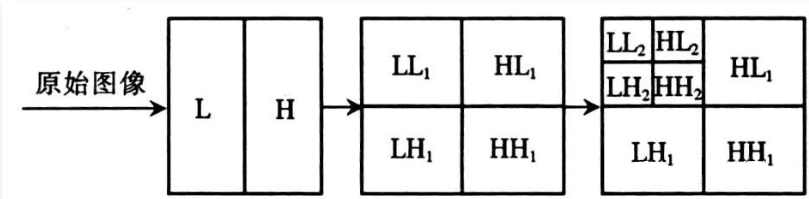
\includegraphics[scale=0.25]{img/wavelet.png}
	\caption{一次小波分解的过程}\label{Wavelet_Process_Image}
\end{figure}
图\ref{Wavelet_Solution_Image}表示一张图像一次小波分解后的结果,其中\ref{wavelet_a}代表低频信息,
\ref{wavelet_h}代表水平方向高频信息,\ref{wavelet_v}代表竖直方向高频信息,\ref{wavelet_d}代表
对角线方向高频信息。\par
\begin{figure}[ht!]
	\centering
	\subcaptionbox{\label{wavelet_a}}{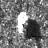
\includegraphics[scale=1]{img/wavelet-a.jpg}}
	\subcaptionbox{\label{wavelet_h}}{
\includegraphics[scale=1]{img/wavelet-h.jpg}}
	\subcaptionbox{\label{wavelet_v}}{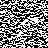
\includegraphics[scale=1]{img/wavelet-v.jpg}}
	\subcaptionbox{\label{wavelet_d}}{
\includegraphics[scale=1]{img/wavelet-d.jpg}}
	\caption{对一张图像进行一次小波分解后的结果}\label{Wavelet_Solution_Image}
\end{figure}
小波图像分解融合算法在很多重要的图形处理库都有实现,比如OpenCV,MATLAB的图像处理包等。\par
NSCT图像分解方法\cite{NSCT_Merge}是在小波分解基础上,基于金字塔分解滤波器和非下采样方向滤波器,对图像进行
高低频和方向面的分解。首先,使用金字塔分解滤波器多次分解图像,得到低频和高频信息。然后,对分解后的高频分量进行
方向分解,分解成为不同方向上的细节信息。图\ref{NSCT_Demo}展示了NSCT的原理,其中\ref{nsct_a}展示了多层分
解示例,\ref{nsct_b}展示了多方向分解示例。\par
\begin{figure}[ht!]
	\centering
	\subcaptionbox{\label{nsct_a}}{\includegraphics[scale=0.25]{img/nsct_a.jpg}}
	\subcaptionbox{\label{nsct_b}}{\includegraphics[scale=0.25]{img/nsct_b.jpg}}
	\caption{NSCT示例}\label{NSCT_Demo}
\end{figure}
NSCT图像分解方法相比小波图像分解方法,可以更加精细地分解图像,更好地保留出高频信息(比如图像中的线,边缘等信息),
同时避免了信号变化极大的时候容易出现的振荡现象。\par
NSCT图像处理算法成熟的实现目前只有随该分解方法论文附带的MATLAB处理库\cite{NSCT_MATLAB}。图\ref{NSCT_Solution_Image}展示其分解后的
状况,其中\ref{nsct_level1}表示第一层的低频信息,\ref{nsct_level2}表示第二层分解的高频信息,\ref{nsct_level3_1}和\ref{nsct_level3_2}
表示第三层分解的高频信息,\ref{nsct_level4_1}、\ref{nsct_level4_2}、\ref{nsct_level4_3}、\ref{nsct_level4_4}、\ref{nsct_level4_5}、
\ref{nsct_level4_6}、\ref{nsct_level4_7}、\ref{nsct_level4_8}表示第四层分解的高频信息。
由图可知,该分解方法能够保留更多高频信息。\par
\begin{figure}[ht!]
	\centering
	\subcaptionbox{\label{nsct_level1}}{\includegraphics[scale=0.4]{img/nsct/level1.jpg}}
	\subcaptionbox{\label{nsct_level2}}{\includegraphics[scale=0.4]{img/nsct/level2.jpg}}
	\subcaptionbox{\label{nsct_level3_1}}{\includegraphics[scale=0.4]{img/nsct/level3_1.jpg}}
	\subcaptionbox{\label{nsct_level3_2}}{\includegraphics[scale=0.4]{img/nsct/level3_2.jpg}}
	\subcaptionbox{\label{nsct_level4_1}}{\includegraphics[scale=0.4]{img/nsct/level4_1.jpg}}
	\subcaptionbox{\label{nsct_level4_2}}{\includegraphics[scale=0.4]{img/nsct/level4_2.jpg}}
	\subcaptionbox{\label{nsct_level4_3}}{\includegraphics[scale=0.4]{img/nsct/level4_3.jpg}}
	\subcaptionbox{\label{nsct_level4_4}}{\includegraphics[scale=0.4]{img/nsct/level4_4.jpg}}
	\subcaptionbox{\label{nsct_level4_5}}{\includegraphics[scale=0.4]{img/nsct/level4_5.jpg}}
	\subcaptionbox{\label{nsct_level4_6}}{\includegraphics[scale=0.4]{img/nsct/level4_6.jpg}}
	\subcaptionbox{\label{nsct_level4_7}}{\includegraphics[scale=0.4]{img/nsct/level4_7.jpg}}
	\subcaptionbox{\label{nsct_level4_8}}{\includegraphics[scale=0.4]{img/nsct/level4_8.jpg}}
	\caption{NSCT四层分解实例}\label{NSCT_Solution_Image}
\end{figure}
\subsection{图像融合方法}
图像融合方法是根据图像特征融合图像的过程,包括图像特征提取、图像分解信息融合和图像分解方法逆变换。接下来介绍基于
不同的图像特征实现的图像融合方法,包括最大绝对值融合法、主成分变换融合法和核范式加权融合法。\par
最大绝对值融合法是逐像素来进行融合的方法,目标是将每个图像中最突出的信息集中到最终融合图像中,从而提高最终图像的
信息量。具体来说,该方法逐像素进行融合,选择每个位置上绝对值最大的像素作为最终融合图像的对应像素。在黑白影像中,
像素的亮度通常用八位无符号整数来表示。公式如下:
\begin{equation}w_{dk}^{i,j}=max\left(\{\left|w_{dn}^{i,j}\right|,n\in\left[1,K\right],n\in N^\ast\}\right)\end{equation}
其中,$w_{dk}^{i,j}$表示最终融合图像在位置$(i,j)$处的像素值,$w_{dn}^{i,j}$表示第$n$张图像在在位置$(i,j)$
处的像素值,$K$表示输入的图像数量。算法描述如\ref{max_abs_algorithm}所示。\par
\IncMargin{2em}
\begin{algorithm}[H]
	\SetKwData{Left}{left}\SetKwData{This}{this}\SetKwData{Up}{up}
	\SetKwInOut{KwIn}{输入}\SetKwInOut{KwOut}{输出}
	\SetKwFunction{Union}{Union}\SetKwFunction{FindCompress}{FindCompress}
	\KwData{一系列相同大小的图像矩阵$Im$,大小是$w\times l$,数量是$length$}
	\KwResult{融合后的图像矩阵$I$}
	将$I$设置为$w\times l$的全0矩阵\;
	\For{$i\leftarrow w$}{
		\For{$j\leftarrow l$}{
			$value\_array \leftarrow$长度为$length$的数组\;
			\For{$pic\leftarrow length$}{
				$value\_array[pic] \leftarrow Im[pic][i][j]$的绝对值\;
			}
			$I[i][j] \leftarrow value\_array$中的最大值\;
		}
	}
	\caption{最大绝对值融合法}\label{max_abs_algorithm}
\end{algorithm}
\DecMargin{2em}
主成分变换融合法利用了图像的主成分分析原理来合成图像。这种方法不仅基于主成分变换的理论基础,还巧妙地结合了图像
的低频信息,以实现更加精确和有效的图像融合效果。\par
主成分变换(Principal Component Analysis, PCA)是一个常用的数据降维算法\cite{PCA},通过这个算法,可以
提取出数据的特征。该算法主要是从数据原始空间中寻找到若干“坐标轴”来表示数据特征,其中,第一个坐标轴表示原始数据
方差最大的方向;第二个坐标轴是与第一个坐标轴正交的平面中,方差最大的;第三个是与前两个轴正交平面中方差最大的,
以此类推。这些坐标轴可以作为图像特征的一部分,同时很多数据特征都集中在前几个“坐标轴”中。\par
根据论文\parencite{PCA_Merge},本方法将图像的低频信息进行主成分变换,将第一个分量作为新的近似低频信号。之后,
将近似低频信号和高频信号按照公式\ref{PCA_1}进行加权:
\begin{equation}
	HH(x,y)=\sum_{i=1}^{N}k_iHH_i(x,y),\space k_i=\mu_i/\sum_{i=1}^{N}\mu_i
	\label{PCA_1}
\end{equation}
其中,$\mu_i$表示第$i$个图像的数据平均值,$HH_i(x,y)$表示需要融合的第$i$个图像,$HH(x,y)$表示融合后的图像。
算法描述如\ref{pca_algorithm}所示。\par
\IncMargin{2em}
\begin{algorithm}[H]
	\SetKwData{Left}{left}\SetKwData{This}{this}\SetKwData{Up}{up}
	\SetKwFunction{Union}{Union}\SetKwFunction{FindCompress}{FindCompress}
	\SetKwInOut{KwIn}{输入}\SetKwInOut{KwOut}{输出}
	\KwData{一系列相同大小的图像矩阵$Im$,大小是$w\times l$,数量是$length$;长度为$length$的数组$value\_array$}
	\KwResult{融合后的图像矩阵$I$}
	对$Im$里图像逐个进行图像分解方法,获得图像的低频信息$Ilow$和高频信息$Ihigh$\;
	$Inewlow, Inewhigh\leftarrow$ 融合后的低频信息和高频信息\;
	\For{$It\leftarrow Ilow, Ihigh$}{
		\If(低频信息进行主成分变换或得权重){${It}=={Ilow}$}{
			\For{$i\leftarrow length$}{
				$pca\_level \leftarrow$ $Ilow[i]$ 长宽高的最小值 $ * 0.75$\;
				$Ilow[i] \leftarrow$ 对 $Ilow[i]$ 进行 $pca\_level$ 层主成分变换的结果\;
				$value\_array\leftarrow Ilow[i]$ 所有值的平均值\;
			}
			$value\_array \leftarrow value\_array / value\_array$ 的总和\;
			\For{$j\leftarrow length$}{
				$Inewlow\leftarrow Ilow[j] * value\_array[j]$\;
			}		
		}
		\For{$j\leftarrow length$}{
			$Inewhigh\leftarrow Ihigh[j] * value\_array[j]$\;
		}
	}
	对 $Inewlow$ 和 $Inewhight$ 进行逆变换\;
	\caption{主成分变换融合法}\label{pca_algorithm}
\end{algorithm}
\DecMargin{2em}
核范式加权融合法基于矩阵的核范式信息,结合图像低频信息得出的图像合成算法。\par
核范式(Nuclear Norm)是指矩阵的所有奇异值之和,其中用于约束矩阵的低秩性质\cite{Nuclear_Norm}。对于稀疏性
数据,矩阵通常是低秩的且包含大量冗余信息,这些信息可用于数据恢复和特征提取。对于黑白图像矩阵,可以通过对该矩阵进
行奇异值分解或得该图像的奇异值,奇异值累加后获得核范式。\par
根据论文\parencite{Softmax_Merge},本方法需要逐张分析图像的核范式,从而获得融合图像的权重。根据权重融合最终
的图像。该方法的权重公式如下:
\begin{equation}w_{dk}^{i,j}=\frac{w_{dk}^{\hat{i},j}}{\sum_{q=1}^{K}w_{dq}^{\hat{i},j}}\end{equation}
\begin{equation}w_{dk}^{\hat{i},j}={\left\| re\left(V_{dk}^{i,j}\right)\right\|}_*\end{equation}
其中,$re\left(V_{dk}^{i,j}\right)$表示需要重构的图像,$\cdot_*$表示该图像的核范式,$K$表示输入的图像数量。
本算法描述如\ref{neclear_algorithm}所示。\par
\IncMargin{2em}
\begin{algorithm}[H]
	\SetKwData{Left}{left}\SetKwData{This}{this}\SetKwData{Up}{up}
	\SetKwFunction{Union}{Union}\SetKwFunction{FindCompress}{FindCompress}
	\SetKwInOut{KwIn}{输入}\SetKwInOut{KwOut}{输出}
	\KwData{一系列相同大小的图像矩阵$Im$,大小是$w\times l$,数量是$length$}
	\KwResult{融合后的图像矩阵$I$}
	将$I$设置为$w\times l$的全0矩阵\;
	$value\_array\leftarrow$ 长度为$length$的数组\;
	\For{$i\leftarrow length$}{
		$value\_array \leftarrow Im[i]$经过SVD分解后获得的奇异值\;
	}
	$value\_array$的每个元素除以$value\_array$的总和\;
	\For{$j\leftarrow length$}{
		$Inewlow\leftarrow Ilow[j] * value\_array[j]$\;
	}		
	\caption{核范式加权融合法}\label{neclear_algorithm}
\end{algorithm}
\DecMargin{2em}
\subsection{融合结果量化评估指标}\label{evaluation_subsection}
当涉及到融合后的图像时,仅凭人眼的主观判断确实不够。为了更客观地评估图像融合的质量,本毕设引入了一些量化指标来衡量
融合图像的质量。以下介绍本毕设涉及的量化指标\cite{Eval}:\par
\begin{enumerate}
\item \textbf{熵值}。图像的熵值(entropy)代表了图像所包含的信息量。具体定义为:
\begin{equation}EN=-\sum_{i=0}^{L-1}p_ilog_2p_i\end{equation}
其中$L$代表灰度级数,$p_i$代表图像灰度级的直方图。其值越大,表示图像包含的信息越多。\par
\item \textbf{标准差}。图像的标准差(Standard Deviation, SD)表示图像信息的离散程度,其公式如下:
\begin{equation}SD=\sqrt{\sum_{i=1}^{M}\sum_{j=1}^{N}(F(i,j)-\mu)^2}\end{equation}
其中$\mu$表示图像的均值。其值越大,表示数据离散程度越高,图像越能突出表示特征。
\item \textbf{互信息}。融合后的图像和融合前图像的互信息(Mutual Information)表示融合前后图像信息的相关性,该值越大越能表示相关性越强。
\item 图像的\textbf{空间频率}(Spatial Frequency, SF)是通过测量融合图像的梯度分布,揭示融合图像的细节和纹理信息的指标。具体定义为
\begin{equation}SF = RF^2 + CF^2\end{equation}
式中, $RF$表示行频率,$CF$表示列频率,他们的计算方式分别如下:
\begin{equation}RF = \sqrt{\sum_{i=1}^{M}\sum_{j=1}^{N}(F(i,j)-F(i,j-1))^2}\end{equation}
\begin{equation}CF = \sqrt{\sum_{i=1}^{M}\sum_{j=1}^{N}(F(i,j)-F(i-1,j))^2}\end{equation}
更高的空间频率意味着更加丰富的边缘和纹理细节。
\end{enumerate}
\section{MATLAB程序环境}
本段介绍本毕设涉及到的MATLAB以及雷达仿真工具箱。
\subsection{MATLAB}
MATLAB(Matrix Laboratory,矩阵实验室)是由美国 The MathWorks 公司出品的商业数学软件。
它是一种用于算法开发、数据可视化、数据分析以及数值计算的高级技术计算语言和交互式环境。本软件
主要用于数值运算,但利用众多附加工具箱,它也适用于不同领域的应用,例如控制系统设计与分析、影
像处理、深度学习、信号处理与通讯、金融建模和分析等。截至2020年,全球有超过400万用户使用MATLAB,
涵盖工程、科学和经济学等领域。
\subsection{MATLAB图形化界面设计器}
MATLAB图形化界面设计器是一个交互式开发环境,用于设计应用程序的布局并编写其行为。其拥有大量的组件
库,和MATLAB集成良好,可用于图形用户界面设计。\par
本设计器可以通过拖放可视组件,来很方便地设计图形用户界面的布局。同时,其集成了代码编辑器,可以快速
编写应用程序的行为,同时自动检查代码问题。通本程序还可以使用状态图模式来建模应用程序的行为。\par
本设计器提供丰富的组件和自定义交互,不仅拥有标准组件(如按钮、复选框、树状列表和下拉列表),还可以
使用仪表、灯、旋钮和开关等控件来模拟仪表板的外观和操作。此外,本程序还拥有大量容器组件(如选项卡、
面板和网格布局)来组织用户界面。\par
通过这个部件,使用者可以快速创建桌面应用程序,或Web应用程序,并与其他用户共享。同时,面对以前使用
GLIDE设计的软件,该程序可以快速将其迁移到设计器开发环境,在保留老软件的兼容性同时方便用户快速集成。\par
\subsection{MATLAB雷达仿真工具箱}
MATLAB雷达仿真工具是在2021年由美国MathWorks公司发布的雷达仿真工具,其中包括了设计、仿真、分析和
测试多功能雷达系统的算法和工具。通过该工具,用户可以设计、模拟、分析和测试多功能雷达系统,进而加速
项目的验证和落地。目前,该工具在汽车雷达仿真、合成孔径雷达仿真、以及机载雷达设计方面得到了广泛应用。
\chapter{系统设计与实现}
本章在上一章背景的基础上,介绍了使用MATLAB平台实现本毕设的流程。首先,本毕设依托MATLAB雷达仿真
平台,仿真模拟了合成孔径雷达对模拟地形上的目标进行成像的流程,获得了仿真模拟数据。然后,基于背景
里提到的图像分解方法和融合方法,实现了一些图像融合算法,同时实现了融合图像量化评估指标。最后,本
毕设将仿真模拟流程和图像融合算法进行整合,添加了用户输入模块和命令行为主的用户操作界面,实现了合
成孔径雷达图像融合软件。
\section{仿真模拟合成孔径雷达}\label{simulation_big_section}
本小节介绍仿真合成孔径雷达的实现过程。其中包括仿真雷达扫描模拟地形,仿真模拟数据的处理。目标是对
模拟地形上的目标点进行多角度成像。具体仿真流程如下:
\begin{compactenum}
	\item 初始化地形,设置放射率,放置目标点。
	\item 设置雷达仿真环境,设置地形数据和目标点数据。
	\item 初始化雷达信息,在仿真环境中设置仿真雷达信息。
	\item 计算雷达位置和目标点位置的夹角,将其作为雷达天线夹角。
	\item 根据用户输入的角度,设置雷达的路径,然后进行模拟回波处理,从而获得仿真成像数据。
	\item 对仿真回波数据进行处理,形成单视复合(SLC)图像数据。
\end{compactenum}\par
该实现过程参考了MATLAB官方示例\cite{SAR_Simulation}。
\subsection{随机地形生成}
随机地形生成过程是在三维坐标轴上面,使用随机数生成用于模拟扫描成像的地形信息。地形包括位置,大小和海拔。
在生成地形的时候,需要地形在三维坐标轴上的位置,初始海拔和海拔最高点,生成的迭代次数,地形粗糙值以及雷达
信号反射率。生成的迭代次数指生成地形时候调用随机数的次数,次数越多,地面越平滑,但过多迭代次数会导致地形
过于平坦。地形粗糙值表示地形丘陵地形的比例,粗糙值越小,生成的地形越粗糙,粗糙值越大,生成的地形越平滑。
雷达信号反射率表示地表对雷达信号的反射能力。仿真平台本身预设了诸如丘陵,森林等地形的反射值,本模拟需要设置
海拔和反射率的关系。随机地形生成步骤如下:
\begin{compactenum}
	\item 根据输入的坐标轴范围,获取变化率,生成地形生成范围。
	\item 根据初始海拔,平均海拔和之前设置的高度数据(如果不是第一次),生成固定大小的高度信息。
	\item 将海拔小于0的部分设为0。
	\item 根据设置的迭代次数,重复第2步和第3步。
	\item 将高度信息放缩到地形生成范围内,返回坐标轴和高度信息。
	\item 在地形上设置信号反射率。
\end{compactenum}\par
本仿真将在X轴$[900, 1600]$范围,Y轴$[-400, 400]$范围内生成地形。其粗糙值为1.5,最高海拔
100米,初始海拔0米,循环次数为8次。在生成地形中,高于40米的地形设为丘陵森林的反射率,小于40米
的设为森林的反射率。
\subsection{目标点放置}
为了便于对仿真模拟结果进行分辨,从而进行进一步融合分析,需要进行目标点放置。目标点的放置步骤如下:\par
\begin{compactenum}
	\item 初始化一个三列矩阵,分别代表三维坐标轴的坐标值。然后将坐标数据填入其中,高度设为0米。
	\item 使用坐标轴找到地形上的对应位置,根据该位置设定高度。
\end{compactenum}\par
在本仿真中,目标点将会放在$(1000,0)$为中心的位置。
\subsection{模拟雷达参数}
考虑到软件使用平台的运行速度,以及模拟成像的分辨率,在本毕设多次尝试后,决定基于L波段雷达仿真数据,
该雷达参数如表\ref{Radar_Parameter_Table}所示。\par
\begin{table}[ht!]
	\begin{center}
		\caption{仿真雷达参数}\label{Radar_Parameter_Table}
		\begin{tabular}{|c|c|}
			\hline
			参数 & 数值 \\
			\hline
			波长 & 1 GHz \\
			\hline
			信号带宽 & 30 MHz \\
			\hline
			脉冲宽度 & 0.003 ms  \\
			\hline
			采样频率 & 60 MHz \\
			\hline
			脉冲重复频率 & 500 Hz \\
			\hline
			天线长度 & 6 m \\
			\hline
			天线宽度 & 0 m \\
			\hline
		\end{tabular}
	\end{center}
\end{table}
\vspace{-1em} 
该参数代表了一个L波长的合成孔径雷达,其方位向分辨率大致5米。雷达的天线长度设定为6米,同时
为保证成像范围较宽,宽度设定为0米。雷达将会在距离地面1000米的高度运行。根据计算,其测距分
辨率大致为5米,方位向分辨率大致2米,其扫描范围大致长100米,宽70米。仿真地形概览如图\ref{terrain_image}所示,
其中红点表示目标点。
\begin{figure}[!htb]
	\centering
	\includegraphics[scale=0.35]{img/terrian.png}
	\caption{仿真地形概览}\label{terrain_image}
\end{figure}
\subsection{雷达运动轨迹}
本毕设参考了由论文\parencite{SAR_Observation_Model}提出的SAR雷达协作监测模型,该模型如图\ref{observation_model_image}
所示,其中$O$代表目标,$Sat_{N}$表示用于监测目标点的合成孔径雷达卫星,$N$代表雷达卫星数量,$Hstar$代表雷达运行高度。本毕设参考
SAR雷达协作监测模型,并结合本毕设多角度合成孔径雷达成像的需求,设计了本毕设中雷达的路径。\par
\begin{figure}[ht!]
	\centering
	\includegraphics[scale=0.35]{img/observation_model.jpg}
	\caption{SAR雷达协作监测模型概览}\label{observation_model_image}
\end{figure}\par
根据3.1.2节的描述,成像中心点在$(1000,0)$的位置。根据数据推算的辐照带大小,雷达将在距离地形上1000米位置成像。考虑到雷达运行
高度和雷达与目标点的距离,雷达天线大致和地形平面法线成45度角。与此同时,考虑到雷达是侧视成像,成像大小需要表示200米,雷达需要
按照每秒100米的速度运行两秒时间。\par
同时,由于模拟涉及到对目标点的多角度成像,需要用户输入成像时候角度。\par
综上所述,本毕设的路径中点将在以$(1000,0)$为中心的圆上。其路径也将与该圆半径相切,长度为400米。同时,规定$(0,0)$为0度的成像
路径中点。路径示例如图\ref{radar_route_image}所示,其中绿点代表雷达,黑色线条代表运行路径,红点代表雷达开始位置。
\begin{figure}[ht!]
	\centering
	\includegraphics[scale=0.4]{img/radar_route.png}
	\caption{0度成像的轨迹概览}\label{radar_route_image}
\end{figure}\par
在路径方面,涉及到路径的动态运算。所以,需要用户提供成像角度,然后计算目标点的起始点和结束点。根据图\ref{radar_route_image},
路径计算算法在算法\ref{route_calculation_algorithm}里面描述。\par
\IncMargin{2em}
\begin{algorithm}[H]
	\SetKwData{Left}{left}\SetKwData{This}{this}\SetKwData{Up}{up}
	\SetKwFunction{Union}{Union}\SetKwFunction{FindCompress}{FindCompress}
	\SetKwInOut{KwIn}{输入}\SetKwInOut{KwOut}{输出}
	\KwData{成像的角度$\theta$,路径中点$(x_0,y_0)$,旋转参考点$(x,y)$,雷达运行速度$v$,运行时间$dur$}
	\KwResult{路径的起点$(x_{start},y_{start})$和终点$(x_{end},y_{end})$}
	$x_{mid} \leftarrow x + (x_0 - x) * \cos(\theta) - (y_0 - y) * \sin(\theta)$\;
	$y_{mid} \leftarrow y + (y_0 - y) * \cos(\theta) + (x_0 - x) * \sin(\theta)$\;
	$x_{start} \leftarrow x_{mid} + (v * dur * \sin(angle))/2 $\;
	$y_{start} \leftarrow y_{mid} + (v * dur * \cos(angle))/2 $\;
	$v_x \leftarrow v * sin(\theta)$\;
	$v_y \leftarrow v * cos(\theta)$\;
	$x_{stop} \leftarrow x_{start} + v_x * dur $\;
	$y_{stop} \leftarrow y_{start} + y_x * dur $\;
	\caption{路径起点终点计算}\label{route_calculation_algorithm}
\end{algorithm}
\DecMargin{2em}
\subsection{模拟回波处理}
根据上面得到的信息,本毕设创建了一个合成孔径雷达仿真模拟环境。而合成孔径雷达成像的关键,是对回波的模拟接收和处理。\par
在模拟环境中通过模拟,会得到回波脉冲。回波脉冲数量设为$num_{p}$,其计算公式如下:
\begin{equation}num_{p} = \frac{dur}{T} + 1\end{equation}
其中,脉冲重复间隔$T$是根据脉冲重复频率$f_{pr}$来计算的,公式为:
\begin{equation}T=1/f_{pr}\end{equation}\par
在获得脉冲后,需要对每一个脉冲进行采样。在合理的范围内对脉冲进行采样,能够在保留脉冲信息的同时,节省数据空间量。采样限制
可以在采样范围和采样数量上面进行处理。在本模拟,采样范围设置为$\left[500,2500\right]$。\par
采样数量$num_{s}$与最大采样范围所代表的脉冲传播时间进行计算相关,计算公式如下:
\begin{equation} num_{s}=2*\frac{m}{c}*f_{s} \end{equation}
其中,$c$代表光速,$f_{s}$代表采样频率,$m$代表最大采样范围。\par
在获取这些信息的基础上,执行雷达运行的仿真过程。这一过程涉及模拟雷达发射和接收脉冲信号的动态行为。每一次雷达发射脉冲后,
都会接收到从地面反射回来的回波信号,这些信号携带了地形特征和目标物体的信息。\par
对于每次接收到的雷达脉冲回波,模拟流程会将其信息存储在一个预先定义好的矩阵中。这个矩阵的长为采样数量,高为脉冲数量,每
个元素代表一个特定时间和空间位置的回波信号强度。随着雷达平台的移动和扫描,矩阵逐渐被填充,直至覆盖了整个成像区域。\par
这些原始回波信息并不直接等同于我们最终想要得到的图像。为了将这些数据中转换为雷达扫描图像,在回波信息的基础上,需要通过
后续处理以获得最终图像。
\subsection{数据保存}
模拟回波数据是一个复数矩阵。复数的模长能够描述该点的信号强度,为了获得成像结果,需要将该矩阵转换为以模长为数据的矩阵。在此
之后,根据雷达的运行轨迹和分辨率对图像大小进行调整,使其能够反应地貌和目标点状态。这些参数是根据雷达的波长,采样频率,以及
运行轨迹决定的。处理原始信息的算法如算法\ref{deal_radar_raw_algorithm}所示,该算法根据采样频率计算图片的高度,根据采
样率和雷达运行速度计算图片宽度。\par
\IncMargin{2em}
\begin{algorithm}[H]
	\SetKwData{Left}{left}\SetKwData{This}{this}\SetKwData{Up}{up}
	\SetKwFunction{Union}{Union}\SetKwFunction{FindCompress}{FindCompress}
	\SetKwInOut{KwIn}{输入}\SetKwInOut{KwOut}{输出}
	\KwData{图像矩阵$A$, 最小采样率$min_s$, 雷达运行速度$v$, 采样频率$f_s$, 脉冲重复频率$f_{pr}$}
	\KwResult{放缩后的图像矩阵$I$}
	$n_{p} \leftarrow A$ 的高度 \;
	$d_u \leftarrow v/f_{pr}$ \;
	$d_{ky} \leftarrow 2\pi /n_{p}*du$ \;
	$d_y \leftarrow 2\pi / n_{p}*d_{ky}$ \;
	$y \leftarrow dy * n_{p}$ \;
	$n_{s} \leftarrow A$ 的宽度 \;
	$samples \leftarrow [min_s, min_s + n_s - 1] $\;
	$t_{s} \leftarrow samples / f_s $\;
	$rngVec \leftarrow $通过光速和采样时间获取长度范围\;
	$x \leftarrow rngVec$最大值和最小值的差\;
	$I \leftarrow A$矩阵逐元素计算绝对值,然后转置\;
	$I \leftarrow $将图像 $I$ 按照长 $x$ 宽 $y$ 的设定重新放缩\;
	\caption{图像后期放缩方法}\label{deal_radar_raw_algorithm}
\end{algorithm}
\DecMargin{2em}
在获取图像之后,图像只有一小部分有显像,这是因为雷达辐照带的视场限制,导致目标成像只占据回波的一小部分。
为了去除无效信息,需要对上述成像结果进行裁剪处理,从而获取最终的图像。
\subsection{仿真结果}\label{simulation_result_subsection}
通过上述的模拟步骤,图\ref{simulation_result_image}是在地形生成随机数为5000的情况下的模拟成像的
结果。其中,a和e是正负6度路径的成像结果,b和d是正负3度路径的成像结果,c是0度路径的成像结果。\par
\begin{figure}[!htb]
	\centering
	\subcaptionbox{\label{simulation_-6}}{\includegraphics[scale=0.6]{img/simulation/pic-6-5000.jpg}}
	\subcaptionbox{\label{simulation_-3}}{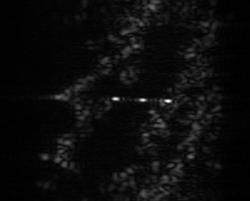
\includegraphics[scale=0.6]{img/simulation/pic-3-5000.jpg}}
	\subcaptionbox{\label{simulation_0}}{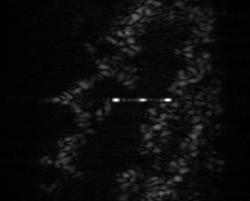
\includegraphics[scale=0.6]{img/simulation/pic0-5000.jpg}}
	\subcaptionbox{\label{simulation_3}}{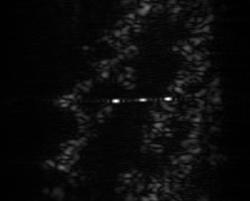
\includegraphics[scale=0.6]{img/simulation/pic3-5000.jpg}}
	\subcaptionbox{\label{simulation_6}}{\includegraphics[scale=0.6]{img/simulation/pic6-5000.jpg}}
	\caption{仿真模拟成像结果}\label{simulation_result_image}
\end{figure}
在本毕设编程使用的苹果公司Mac Mini 2023电脑上,每张仿真SAR图像生成的平均耗时为5分钟。耗时中,
绝大多数时间是被仿真模拟雷达回波所占据。如果雷达天线缩短,虽然能提高分辨率,但是采样也同样添加了,
由于仿真生成了更多的采样数据,仿真时间耗时会更长。在本毕设中,将雷达天线从6米缩短到3米,成像时间
将达到30分钟,这样长的时间对于实际应用过于缓慢。
\section{图像融合算法}\label{merge_algorithm_section}
本小节介绍本毕设中图像融合算法的实现,其本质是对第二章中涉及到的图像融合算法使用MATLAB进行实现。
单张合成孔径雷达成像所包含的信息比较少,通过对多角度合成孔径雷达图像进行融合,合成孔径雷达成像的
信息量将会得到提升,从而有助于进一步应用图像,比如在定位等。\par
在实现融合算法后,本毕设将对\ref{simulation_result_subsection}节的仿真结果进行融合,并对融
合图像进行量化评估,从而得出融合算法的特点。对融合图像的量化评估指标实现完全参考\ref{evaluation_subsection}中
提到的量化指标进行实现,这里不再赘述。需要注意的是,无论本毕设对算法的评估结果如何,这些算法都将集成到最终
的图像融合软件中,提供给用户使用。\par
下图展示用于融合的图像,这些图像是基于图\ref{simulation_result_image}进行预处理得到的。其中,
a和e是正负6度路径的成像结果,b和d是正负3度路径的成像结果,c是0度路径的成像结果。
\begin{figure}[!htb]
	\centering
	\subcaptionbox{\label{dealt_-6}}{\includegraphics[scale=1]{img/simulation/pic-6-5000.jpg_dealt.jpg}}
	\subcaptionbox{\label{dealt_-3}}{\includegraphics[scale=1]{img/simulation/pic-3-5000.jpg_dealt.jpg}}
	\subcaptionbox{\label{dealt_0}}{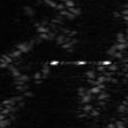
\includegraphics[scale=1]{img/simulation/pic0-5000.jpg_dealt.jpg}}
	\subcaptionbox{\label{dealt_3}}{\includegraphics[scale=1]{img/simulation/pic3-5000.jpg_dealt.jpg}}
	\subcaptionbox{\label{dealt_6}}{\includegraphics[scale=1]{img/simulation/pic6-5000.jpg_dealt.jpg}}
	\caption{经过预处理步骤处理的仿真结果}\label{simulation_dealt_image}
\end{figure}\par
以下介绍本毕设里实现的图像融合算法。\par
\subsection{STRAIGHT法}
本法是一次小波分解,最大绝对值融合法的结合。小波变换是最广泛使用的图像分解算法,故将其作为分解图像
的参照组。同时,最大绝对值融合法的编程和运算相对简单,故将其作为融合时候的参照组。这个方法作为融合
图像算法的对照组,用于和下面算法作出基准对比。本方法步骤如下:\\
\begin{enumerate*}[itemjoin=\\\hspace*{\parindent}, itemsep=5mm\hspace*{\parindent}]
	\item 输入图像逐个进行一次小波分解,得到图像的低频信息和水平方向、竖直方向和对角线方向的高频信息。
	\item 对分解信息进行最大绝对值融合法图像融合。
	\item 将融合的信息使用小波变换的逆变换,完成融合步骤。
\end{enumerate*}\par
图\ref{simulation_straight}展示了由STARIGHT法融合的图像结果。
\begin{figure}[!htb]
	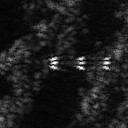
\includegraphics[scale=1]{img/simulation/result_straight.jpg}
	\caption{STARIGHT法融合的图像}\label{simulation_straight}
\end{figure}
\subsection{WT-PCA法}
本法是一次小波分解,主成分变换融合法的结合,参考了论文\parencite{PCA_Merge}。在多层小波分解中,下一
层的分解利用了上一次分解的低频信息,如果输入图像过小,则会导致多层分解后,最底层的低频信息主成分过少,从
而主成分信息过少。在主成分信息过少的情况下,去除主成分信息会导致信息损失过大,从而使第一个主成分分量包含
的信息过少。综上所述,本方法仅会进行一次小波分解,对其低频信息进行主成分变换,并获得其第一个主成分分量。
本方法步骤如下:\\
\begin{enumerate*}[itemjoin=\\\hspace*{\parindent}, itemsep=5mm\hspace*{\parindent}]
	\item 输入图像逐个进行一次小波分解,得到图像的低频信息和水平方向、竖直方向和对角线方向的高频信息。
	\item 图像的低频使用主成分变换法,获取其第一个主成分分量。之后计算这些信息的平均值,获得融合权重。
	\item 根据权重,对图像的低频信息和高频信息进行加权平均融合。
	\item 将融合的信息使用小波变换的逆变换,完成融合步骤。
\end{enumerate*}\par
图\ref{simulation_wavelet_pca}展示了由WT-PCA法融合的图像结果。
\begin{figure}[!htb]
	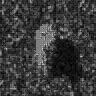
\includegraphics[scale=1]{img/simulation/result_wavelet_pca.jpg}
	\caption{WT-PCA法融合的图像}\label{simulation_wavelet_pca}
\end{figure}
\subsection{WT法}
该方法是三次小波分解,最大绝对值融合法的结合。在多层小波分解中,下一层分解基于上一次分解的低频信息。如
果我们对一张图像进行多层小波分解,并在每一层进行融合,可以提高融合后图像的质量。每一层的低频部分包含更
全局的信息,而高频部分包含更细节的信息。通过多层分解和融合,我们可以更好地保留图像的结构和细节。所以,
本方法决定使用三次小波分解,对分解的低频和高频使用最大值融合法。本方法步骤如下:\\
\begin{enumerate*}[itemjoin=\\\hspace*{\parindent}, itemsep=5mm\hspace*{\parindent}]
	\item 输入图像逐个进行三次小波分解,得到图像的低频信息和高频信息。
	\item 对分解信息进行最大绝对值融合法图像融合。
	\item 将融合信息进行三次小波变换逆变换,完成融合步骤。
\end{enumerate*}\par
图\ref{simulation_wavelet}展示了由WT法融合的图像结果。
\begin{figure}[!htb]
	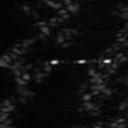
\includegraphics[scale=1]{img/simulation/result_wavelet.jpg}
	\caption{WT法融合的图像}\label{simulation_wavelet}
\end{figure}
\subsection{WT-SOFT法}
本法是三次小波分解,核范式加权融合法的融合。本方法在上一个方法的基础上,对数据量较大的低频信息使用核范式
加权法,对数据量较低的高频信息使用绝对值最大法。核范式加权法使用核函数来对低频信息进行加权,以便更好地保
留图像的结构信息,进而集中数据。而对于高频信息,由于信息量较少,使用核范式融合对最终图像融合效果的提升有
限。而核范式计算时间较长,故高频使用最大值融合法。使用本方法步骤如下:\\
\begin{enumerate*}[itemjoin=\\\hspace*{\parindent}, itemsep=5mm\hspace*{\parindent}]
	\item 输入图像逐个进行三次小波分解,得到图像的低频信息和高频信息。
	\item 对分解信息的低频信息使用核范式加权法,高频信息使用最大绝对值融合法进行融合。
	\item 将融合信息进行三次小波变换逆变换,完成融合步骤。
\end{enumerate*}\par
图\ref{simulation_wavelet_softmax}展示了由WT-SOFT法融合的图像结果。
\begin{figure}[!htb]
	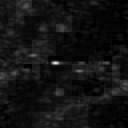
\includegraphics[scale=1]{img/simulation/result_wavelet_softmax.jpg}
	\caption{WT-SOFT法融合的图像}\label{simulation_wavelet_softmax}
\end{figure}
\subsection{NSCT法}\par
本方法是三层NSCT分解,最大绝对值融合法的融合。与小波分解方法相比,NSCT信息将信号或图像分解成多个尺度和
方向的子带。这种分解对比小波分解,在处理图像的边缘和纹理时非常有效,因为它可以捕捉到更丰富的局部结构信息。
本法可和WT法进行比较。本方法步骤如下:\\
\begin{enumerate*}[itemjoin=\\\hspace*{\parindent}, itemsep=5mm\hspace*{\parindent}]
	\item 输入图像逐个进行三层NSCT分解,得到图像的低频信息和高频信息。
	\item 对分解信息进行最大绝对值融合法图像融合。
	\item 对融合后信息进行NSCT逆变换,完成融合步骤。
\end{enumerate*}\par
图\ref{simulation_nsct}展示了由NSCT法融合的图像结果。
\begin{figure}[!htb]
	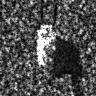
\includegraphics[scale=1]{img/simulation/result_nsct.jpg}
	\caption{NSCT法融合的图像}\label{simulation_nsct}
\end{figure}
\subsection{NSCT-PCA法}
本法是三层NSCT分解,主成分变换融合法的结合。当我们使用 NSCT 进行分解时,它只会生成
一个低频信息子带,因为该分解方法的层级分解主要针对高频信息。为了进一步提取图像的特征,我们可以考虑对NSCT进行
多次分解,然后使用主成分融合法进行加权融合。本方法步骤如下:\\
\begin{enumerate*}[itemjoin=\\\hspace*{\parindent}, itemsep=5mm\hspace*{\parindent}]
	\item 输入图像逐个进行三层NSCT分解,得到图像的低频信息和高频信息。
	\item 图像的低频使用主成分变换法,获取其第一个主成分分量。之后计算这些信息的平均值,获得融合权重。
	\item 根据权重,对图像的低频信息和高频信息进行加权平均融合。
	\item 对融合后信息进行NSCT逆变换,完成融合步骤。
\end{enumerate*}\par
图\ref{simulation_nsct_pca}展示了由NSCT-PCA法融合的图像结果。
\begin{figure}[!htb]
	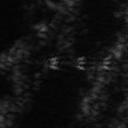
\includegraphics[scale=1]{img/simulation/result_nsct_pca.jpg}
	\caption{NSCT-PCA法融合的图像}\label{simulation_nsct_pca}
\end{figure}
\subsection{NSCT-SOFT法}
本法是三层NSCT分解,核范式加权融合法的结合,对应WT-SOFT法。由于NSCT分解出来的高频信息较少,
高频用最大值融合法比使用核范式方法更能集中信息。故本法低频使用核范式加权法融合,高频使用最大绝对值法。
本方法步骤如下:\\
\begin{enumerate*}[itemjoin=\\\hspace*{\parindent}, itemsep=5mm\hspace*{\parindent}]
	\item 输入图像逐个进行三层NSCT分解,得到图像的低频信息和高频信息。
	\item 对分解信息的低频信息使用核范式加权法,高频信息使用最大绝对值融合法进行融合。
	\item 对融合后信息进行NSCT逆变换,完成融合步骤。
\end{enumerate*}\par
图\ref{simulation_nsct_softmax}展示了由NSCT-SOFT法融合的图像结果。
\begin{figure}[!htb]
	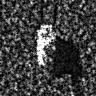
\includegraphics[scale=1]{img/simulation/result_nsct_softmax.jpg}
	\caption{NSCT-SOFT法融合的图像}\label{simulation_nsct_softmax}
\end{figure}
\subsection{图像融合算法的分析}
本小节将会对上述融合图像以熵值、标准差、空间频率,和对原先照片相比较得出的互信息中位数作为量化标准,
对融合结果进行量化评估。融合的量化评估结果如表\ref{simulation_fusion_result}所示。
\begin{table}[ht!]
	\caption{融合结果评估指标一览}\label{simulation_fusion_result}
	\begin{tabular}{|c|c|c|c|c|c|}
		\hline
		序号 & 融合方式 & 图像熵值 & 标准差 & 空间频率 & 互信息中位数 \\
		\hline
		1 & STRAIGHT法 & 5.7255 & 23.4691 & 7.4102 & 1.0584  \\
		\hline
		2 & WT\_PCA法 & 4.9078 & 12.5717 & 3.7736 & 1.1237  \\
		\hline
		3 & WT法 & 5.0306 & 16.0453 & 5.2744 & 0.6776 \\
		\hline
		4 & WT\_SOFT法 & 5.1888 & 15.5258 & 5.3491 & 0.7829  \\
		\hline
		5 & NSCT法 & 5.5952 & 21.1766 & 6.8498 & 0.9387 \\
		\hline
		6 & NSCT\_PCA法 & 5.3152 & 18.9851 & 6.6609 & 0.8365 \\
		\hline
		7 & NSCT\_SOFT法 & 4.9226 & 13.7189 & 3.3753 & 1.1513 \\
		\hline
	\end{tabular}
\end{table}
\vspace{-1em} \par
通过对量化评估结果进行分析,可以对融合算法进行简要的分析:\par
\begin{enumerate*}[itemjoin=\\\hspace*{\parindent}]
	\item 在图像分解方面,使用 NSCT 方法能够比小波融合保留更多的信息量,同时也能保留更多图像共同的信息。此外,对于小波分解,多层分解对于保留图像整体信息是很有必要的。
	\item 主成分变换融合法虽然是步骤最复杂的方法,但融合效果却是最差的。不仅在视觉上图像的模糊现象明显,而且在一系列指标方面都显著低于平均水平。
	\item 绝对值最大法虽然能够体现相对更好的评估指标,但在视觉呈现上,信息有所损失。尤其是针对目标最上面的一处阴影,大多数使用该方法融合的图像都没能体现。因此,STRAIGHT法会导致信息的损失。不过,该方法可以集中信息量,对一些信息量相对较少的信息,比如图像的高频信息,有很好的融合效果。
	\item 核范式权重法能够更好地体现图像之间的权重信息。尤其是在后三个方法上,不仅在指标上都有优势,而且在视觉上,该方法的图像能够保留更多的信息。此外,该融合方法与 NSCT 方法的结合,能够在指标上和完全的绝对值最大法相媲美。
\end{enumerate*}
\section{图像融合软件设计}
经过上面的设计,本毕设实现了仿真模拟多角度SAR图像的生成和图像融合算法。现在需要将上述实现进行整合,
实现合成孔径雷达图像融合软件。本软件将在MATLAB平台上实现,使用命令行为主,图形化组件为辅的呈现方式。\par
考虑到现实中对合成孔径雷达图像的融合需求,需要在本软件中加入用户输入图像功能。所以,本软件有两个
输入来源:用户数据输入和仿真模拟软件。
\subsection{数据输出}
本软件将会将数据输出到文件夹中,该文件夹的名称包括执行类别和生成日期。执行类别包括用户数据输入和
仿真模拟,生成日期是是使用GB/T 7408\cite{ISO_Time}的YYYY-MM-dd HH:mm:ss格式表示的字符串。\par
在数据输出方面,本软件最主要的功能是融合图像,以及对融合后的图像进行评估。这里需要考虑以下问题。
\begin{compactenum}
	\item 如何标识图像输出;
	\item 如何设计图像评估指标输出;
\end{compactenum}\par
对于第一个问题,融合图像输出需要标识图像的融合算法,这里将会在文件名里体现。如果是仿真模拟输出,
需要在文件名中体现生成图像的随机数和角度。\par
对于第二个问题,本程序将在执行结束的时候提供一份日志。该日志表示了本次融合使用的图像融合方法,
同时分别展示图像融合后的评估信息,包括熵值、标准差、空间频率、和融合前图像的互信息等。同时,如果
是用户自行输入图像,则会展示融合图像的数量;如果是仿真模拟输出,则会展示仿真模拟的参数。\par
\subsection{用户操作流程}
为了方便最终用户使用本软件,本毕设需要设计终端输入和操作流程。考虑到本软件包括了两个功能,同时需要
加入用户输入功能,本毕设将根据以下流程图来设计命令行程序。首先,程序会询问用户数据来源。如果数据来
源是用户的图像,则会要求用户输入图像。如果数据来源是仿真模拟程序,则会询问用户生成地形用的随机数和
成像角度。最后,本程序将数据进行融合,并进行融合图像的量化评估。\par
\begin{figure}[!htb]
\centering
\begin{tikzpicture}[font={\sf \small}]
	\def\smbwd{2cm}

	\node (terminal1) at (0,-1) [draw, terminal,
		minimum width=\smbwd,
		minimum height=0.5cm] {开始};

	\node (input_type) at (0,-2) [draw, process,
		minimum width=\smbwd,
		minimum height=0.5cm] {用户输入执行类型};

	\node (decide_type) at (0,-4.5) [draw, decision,
		minimum width=\smbwd,
		minimum height=0.5cm] {是否需要仿真};

	\node (input_simulation) at (3,-6.5) [draw, process,
		minimum width=\smbwd,
		minimum height=0.5cm] {输入角度和随机种子};

	\node (process_simulation) at (3,-7.5) [draw, predproc,
		minimum width=\smbwd,
		minimum height=0.5cm] {进行仿真出图};

	\node (storage_simulation) at (3,-8.5) [draw, storage,
		minimum width=\smbwd,
		minimum height=0.5cm] {保存仿真结果};

	\node (postproc_simulation) at (3,-9.5) [draw, process,
		minimum width=\smbwd,
		minimum height=0.5cm] {用户后期处理图像};

	\node (user_input) at (0,-8) [draw, process,
		minimum width=\smbwd,
		minimum height=0.5cm] {用户输入图像};

	\coordinate (point1) at (0,-10);

	\node (merge_eval) at (0,-10.75) [draw, predproc,
		minimum width=\smbwd,
		minimum height=0.5cm] {图像融合并评估};

	\node (save_result) at (0,-11.75) [draw, storage,
		minimum width=\smbwd,
		minimum height=0.5cm] {保存融合结果};

	\node (terminal2) at (0,-12.75) [draw, terminal,
		minimum width=\smbwd,
		minimum height=0.5cm] {结束};

	\draw[->] (terminal1) -- (input_type) -- (decide_type);
	\draw[->] (decide_type) -| node[above]{是} (input_simulation);
	\draw[->] (input_simulation) -- (process_simulation) -- (storage_simulation) -- (postproc_simulation);
	\draw[->] (decide_type) -- (user_input);
	\draw[->] (postproc_simulation) |- (point1);
	\draw[->] (user_input) -- (point1);
	\draw[->] (point1) -- (merge_eval) -- (save_result) -- (terminal2);
\end{tikzpicture}
\caption{程序流程图}
\end{figure}
需要说明的是,如果是用户自行输入,本程序将默认数据已经经过处理过。这是因为用户应该对自己生成的数据有
比本软件更清晰的认知,能够更好地把握处理的方式。同时,目前公开提供的合成孔径雷达图像在校准和裁剪方面
已经处理过。
\subsection{进度条显示}
进度条提示是为了展示图像仿真生成进度,告知用户仿真的大致剩余时间。\par
通过前面对图像模拟获得回波过程的分析,本毕设决定将获取脉冲数量和总共获取脉冲数量进行比较,从而得出图像合成的
进度。同时,考虑到用户可能会合成多个角度图像,本毕设还需要显示图像合成张数的进度条。因此,我们需要在一个窗口
内显示多个进度条。\par
本毕设选择使用multiWaitbar\cite{MultiWaitBar}库来显示多个进度条,该库可以在一个函数的开头初始化一个
接收器,然后在函数执行过程中,对该接收器进行信息修改,就能在窗口显示进度。接收器是按照名称来区分对应的进度条
的,所以需要在修改信息的时候附带需要修改进度条的名称。\par
在编程过程中,我们需要对仿真获取数据模块的模拟回波部分进行修改。首先,在函数的开头进行初始化,并定义两个进度
条:图像合成进度和图像张数合成进度。\par
\begin{lstlisting}[firstnumber=72]
% Multi wait bar
multiWaitbar( 'CloseAll' );
multiWaitbar( 'Angle process', 0 );
multiWaitbar( 'Generate process', 0);
\end{lstlisting}
在此之后,我们需要在回波处理的时候,传递已经处理的脉冲数量和所有脉冲数量的比值。\par
\begin{lstlisting}[firstnumber=193]
% ii 代表已经处理的脉冲,numPulse 代表处理过的脉冲
multiWaitbar( 'Generate process', (ii - 1)/numPulses);
\end{lstlisting}
以及当一个角度的图像生成完毕后,传递生成完毕图像的数量和需要生成图像数量的比值。\par
\begin{lstlisting}[firstnumber=84]
% i 代表已经生成的图像数量,length(angles) 代表需要生成图像数量
multiWaitbar( 'Angle process', (i-1)/length(angles) );
\end{lstlisting}
\begin{figure}[!htb]
	\centering
	\includegraphics[scale=0.8]{img/progressbar.jpg}
	\caption{进度条示例}
\end{figure}
\subsection{图像后期处理模块}
该模块是为了将仿真生成的图像进行旋转和裁剪处理,以进行后续的图像融合操作。这个模块是为了处理由仿真程序生成的
图像,而用户自行输入的图像,本程序默认已经处理过。另外,由于旋转图像会出现多余信息,并且由上述仿真程序形成的
图像目标点全在中间。所以在本模块,直接编写裁剪图像范围以供使用。\par
经过上处分析,本模块仅需要对旋转角度进行可视化处理,设计界面如图\label{design_image}所示。在窗口中,左面
显示需要旋转图像原先的样子,右面显示图像旋转后的样子。窗口下方是一个滑动条,用于旋转图像,其范围是负180度到
180度。并以45度作为大刻度,5度作为小刻度。开始阶段只显示需要旋转的图像,当操作完滑动条之后,图像旋转的结果
会在右面展示。刻度右面是一个确认按钮,当用户按下这个按钮后,该模块会在输入图像同样的位置保存旋转裁剪后的图像,
并且以dealt作为标识。\par
\begin{figure}[!htb]
	\centering
	\includegraphics[scale=0.26]{img/rotate_design.png}
	\caption{设计页面}\ref{design_image}
\end{figure}
本模块使用MATLAB App Designer设计界面,在设计页面后编写代码,代码分为定义需要用到的变量和GUI组件回调。\par
在变量方面,除了输入的图像和图像名称,还需要存储旋转角度和旋转后的图像概览。由于该设计器是基于面向对象设计范式
的,所以需要在构造函数编写初始化变量相关的操作,其中最主要的是获取需要旋转的图像。同时,在构造函数里面,初始化
旋转角度为0,而旋转后图像概览留空。\par
在回调方面,则需要绑定滑动块和旋转功能,同时编写保存按钮按下后的功能。对于滑动块,则需要在读取滑动块数值的基础
上,调用旋转图像函数实现图像的处理,保存到旋转后的图像概览。最后,将结果展示在窗口右侧。至于保存函数,则需要使用
预先设定的裁剪范围才能看到图像,之后将裁减后的图像存到原先图像同样的目录中。\par
在编写代码后,需要将GUI导出为MATLAB类,这样方便在程序里面进行集成。在本程序仿真模块中,一个角度的仿真图像合成
完毕后,将会调用本模块进行调整。在集成的时候,需要引入waitfor函数,以等待用户完成旋转操作。否则,MATLAB引擎会
在图像旋转模块运行的同时,进行下一个角度图像的仿真生成,导致该模块运行卡顿。\par
\begin{figure}[!htb]
	\centering
	\includegraphics[scale=0.4]{img/rotate_image.png}
	\caption{旋转页面示例}
\end{figure}
\chapter{运行展示}
这里展示本程序的运行说明,说明本程序应该如何使用,同时展示运行一次的结果。运行本程序,需要拥有MATLAB运行环境。
在运行本程序前,需要安装MATLAB图像处理包,MATLAB雷达模拟工具包和MATLAB小波处理包。虽然本程序是命令行为主,但
部分功能有图形化界面,所以一定要在图形界面运行。\par
本毕设在Mac mini 2023上运行,该电脑拥有8核Apple M2芯片,内存16GB,运行macOS Sonama 14.4.1系统。
软件的运行环境为MATLAB R2024a。
\section{选择模式}
在图形化MATLAB的命令行界面中,通过输入sar\_image\_merge来运行本软件。运行之后,命令行界面会出现本软件的版权
信息,同时要求选择图像来源。来源分为两个:
\begin{compactenum}
	\item 用户自行处理过的图像,代号为1
	\item 本论文第\ref{simulation_big_section}节所述仿真过程生成的数据,代号为2。
\end{compactenum}
用户可以输入1或2来代表前述来源,如果输入了其他数字,程序将会报错退出。图\ref{mode_selection}展示了本程序选择运行模式的界面。
\begin{figure}[!htb]
	\centering
	\includegraphics[scale=0.6]{img/running/mode_selection.png}
	\caption{选择模式}\label{mode_selection}
\end{figure}
\section{用户输入模式}
当用户使用第一个选项时,程序进入用户输入模式。该模式下,程序将会读取用户输入的多角度SAR雷达图像,对这些图像进行
融合,并进行量化分析。
\subsection{图像输入}
在图像输入中,用户需要选择多角度雷达图像所在的文件夹。这些图像需要经过预处理,包括配准和裁剪。用户需要确保需要融合
的所有图像都放在同一个文件夹下,以便统一管理和输出,并确保输出位置的一致性。\par
在MacOS系统中,选择文件夹弹窗如图\ref{choose_picture_folder}所示。在其他系统或桌面环境中,弹窗选择图片的窗口
或有不同。\par
\begin{figure}[!htb]
	\centering
	\includegraphics[scale=0.4]{img/running/choose_picture_folder.png}
	\caption{仿真流程输入}\label{choose_picture_folder}
\end{figure}\par
\subsection{选择融合算法}
在用户选择图像路径之后,本程序将会让用户选择图像融合算法。用户选择算法后,程序将会按照用户输入的算法进行图像融合,并对
融合图像进行量化分析。如果用户选择融合算法,程序将会运行所有的图像融合算法,并对融合结果进行量化分析。选择图像融合算法
的界面在图\ref{user_choose_algo}中展示。\par
\begin{figure}[!htb]
	\centering
	\includegraphics[scale=0.4]{img/running/user_choose_algo.png}
	\caption{选择图像融合算法}\label{user_choose_algo}
\end{figure}\par
\subsection{运行输出}
在图像融合并量化分析后,融合图像和量化评估结果都将会保存在根据运行时间生成的新文件夹中。图\ref{user_result}展示了运行
所有算法的结果,其中,log.txt是日志文件,包括融合图像的量化评估结果。图片名称展示了该图片使用的融合算法。\par
\begin{figure}[!htb]
	\centering
	\includegraphics[scale=0.45]{img/running/usermod_result.png}
	\caption{融合运行输出}\label{user_result}
\end{figure}
\subsection{运行结果}
本次使用MSTAR数据集\cite{MSTAR}中的多角度坦克图像进行融合,这些图像都经过了以下预处理:
\begin{compactenum}
	\item 按照图像附带的角度,将图像进行旋转,使目标位于图像中央。
	\item 裁剪图像,去除因旋转而产生的多余信息。
\end{compactenum}\par
图\ref{tank_dealt_image}展示了用于融合的MSTAR数据集图像,图像已经经过旋转裁剪处理。
\begin{figure}[ht!]
	\centering
	\subcaptionbox{\label{tank_1}}{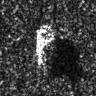
\includegraphics[scale=1]{img/tank/1-cropped.jpg}}
	\subcaptionbox{\label{tank_2}}{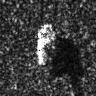
\includegraphics[scale=1]{img/tank/2-cropped.jpg}}
	\subcaptionbox{\label{tank_3}}{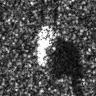
\includegraphics[scale=1]{img/tank/3-cropped.jpg}}\\
	\subcaptionbox{\label{tank_4}}{\includegraphics[scale=1]{img/tank/4-cropped.jpg}}
	\subcaptionbox{\label{tank_5}}{\includegraphics[scale=1]{img/tank/5-cropped.jpg}}
	\caption{需要融合的图像实例}\label{tank_dealt_image}
\end{figure}\par
在预处理后,使用融合算法融合图像,从而获得多角度SAR雷达图像的融合图像。图\ref{tank_merge_result}
展示了对图\ref{tank_dealt_image}进行融合的结果。其中,\ref{tank_straight}代表STRAIGHT法的融合结果,
\ref{tank_straight}代表WT\_PCA法的融合结果,\ref{tank_wavelet}代表WT法的融合结果,\ref{tank_wavelet_softmax}
代表WT\_SOFT法的融合结果,\ref{tank_nsct}代表NSCT法的融合结果,\ref{tank_nsct_pca}代表NSCT\_PCA法
的融合结果,\ref{tank_nsct_softmax}代表NSCT\_SOFT法的融合结果。\par 
\begin{figure}[ht!]
	\centering
	\subcaptionbox{\label{tank_straight}}{\includegraphics[scale=1]{img/tank/result_straight.jpg}}
	\subcaptionbox{\label{tank_wavelet_pca}}{\includegraphics[scale=1]{img/tank/result_wavelet_pca.jpg}}
	\subcaptionbox{\label{tank_wavelet}}{\includegraphics[scale=1]{img/tank/result_wavelet.jpg}}
	\subcaptionbox{\label{tank_wavelet_softmax}}{\includegraphics[scale=1]{img/tank/result_wavelet_softmax.jpg}}
	\subcaptionbox{\label{tank_nsct}}{\includegraphics[scale=1]{img/tank/result_nsct.jpg}}
	\subcaptionbox{\label{tank_nsct_pca}}{\includegraphics[scale=1]{img/tank/result_nsct_pca.jpg}}
	\subcaptionbox{\label{tank_nsct_softmax}}{\includegraphics[scale=1]{img/tank/result_nsct_softmax.jpg}}
	\caption{对图\ref{tank_dealt_image}进行融合的结果}\label{tank_merge_result}
\end{figure}
在此之后,对上述融合图像以熵值、标准差、空间频率,和对原先照片相比较得出的互信息中位数作为量化标准,对
融合结果进行量化评估,从而获得量化评估结果。融合的量化评估结果如表\ref{tank_merge_table}所示。\par
\begin{table}[ht!]
	\caption{用户输入融合结果评估指标一览}\label{tank_merge_table}
	\begin{tabular}{|c|c|c|c|c|}
		\hline
		融合方式 & 图像熵值 & 标准差 & 空间频率 & 互信息中位数 \\
		\hline
		STRAIGHT 法 & 7.4593 & 52.8821 & 13.9746 & 1.9261  \\
		\hline
		WT\_PCA 法 & 6.4928 & 24.7216 & 9.1857 & 1.5282  \\
		\hline
		WT 法 & 7.0148 & 43.9587 & 12.6562 & 1.6993 \\
		\hline
		WT\_SOFT 法 & 7.0204 & 43.7315 & 12.6518 & 1.7007  \\
		\hline
		NSCT 法 & 7.4049 & 53.1878 & 13.6282 & 1.9373 \\
		\hline
		NSCT\_PCA 法 & 6.7062 & 37.0415 & 10.3018 & 1.6980 \\
		\hline
		NSCT\_SOFT 法 & 7.2330 & 51.8677 & 13.5779 & 1.8665 \\
		\hline
	\end{tabular}
\end{table}\par
由此看出,在用户输入图像方面,本程序能够很好地完成合成孔径雷达图像融合工作,并很好地展示各个融合算法的特征。
\section{仿真运行模式}
仿真运行模式是用户运行模式的扩展,和上面的区别为数据来源。这里的数据来源是仿真程序生成的数据。同时,因为仿真运行是有演示
性质的,故所有算法都会被执行。\par
\subsection{输入参数}
用户需要在弹窗中选择输出保存路径。在此之后,用户需要输入成像角度和生成随机地形的随机数,以进行接下来的仿真模拟。成像角度的输
入是按照MATLAB数组的\%start:\%jump:\%end格式来输入的,其中start表示初始的成像角度,jump表示成像角度的增量,end表示最终
的成像角度。随机数则是一个整型变量。输入流程如图\ref{simulation_running}所示。\par
\begin{figure}[!htb]
	\centering
	\includegraphics[scale=0.4]{img/running/simulation_running.png}
	\caption{仿真流程输入}\label{simulation_running}
\end{figure}
\subsection{仿真模拟输出}
当用户输入完毕后,程序将根据运行时间生成一个新的文件夹,并在该文件夹中执行仿真模拟和图像融合。图\ref{simulation_result}
展示了一次仿真模拟的结果。其中,log.txt是日志文件,保存了仿真模拟参数和融合的量化评估结果。仿真模拟图片的文件名中包括成像角
度和随机数,融合图片文件名包括用于融合该图片的融合算法。
\begin{figure}[!htb]
	\centering
	\includegraphics[scale=0.4]{img/running/simulation_result.png}
	\caption{仿真运行结果}\label{simulation_result}
\end{figure}\par
仿真融合结果在本论文\ref{merge_algorithm_section}节中展现,此处不再赘述。由p此可见,本程序不仅能够有效地执行雷达数据的仿真模拟任务,
而且还能成功地实现仿真数据的图像融合,从而清晰地展示每种融合算法的独特属性。
\chapter{总结和展望}
\section{工作总结}
本毕业设计成功开发了一款合成孔径雷达图像融合软件,其核心优势在于能够高效地融合来自不同角度的雷达成像,显著提升图像的整体质量。
该软件不仅简化了多角度合成孔径雷达图像图像的融合过程,还通过仿真模拟合成孔径雷达多角度成像流程,提供了仿真模拟数据,为进一步
的研究提供了便利和支持。\par
在研究的初期阶段,本毕设深入探讨了SAR的成像原理,特别是其侧视成像技术,并详细介绍了SAR的分类、波长参数以及当前广泛使用的仿真
成像软件。这些基础知识的学习为后续的成像仿真实现打下了坚实的基础。此外,本毕设还深入研究了经典的图像融合算法,包括图像分解技术
和融合策略,并在此基础上实现了对图像质量的量化评估方法。\par
在技术实现方面,本毕设选择了MATLAB作为开发平台,并在此平台上完成了软件的构建。通过模拟雷达在不同地形上的多角度扫描,本毕设成功
获取了多角度雷达成像的仿真模拟数据。随后,本毕设实现了多种经典图像融合算法,并完成了对融合后图像的量化评价功能。\par
在软件整合与优化阶段,本毕设整合了多角度成像的仿真模拟与图像融合评估,同时引入了用户输入数据功能,精心设计并优化了用户输入流
程和数据输出格式。这不仅提高了软件的交互性,也增强了其实用性和灵活性。\par
最终,本毕设通过将用户输入的多角度雷达成像数据与仿真模拟的多角度雷达图像进行融合评估,充分展示了本软件能够很好地融合多角度的合成
孔径雷达图像,同时也能很好地仿真多角度合成孔径雷达成像结果。\par
综上所述,本软件不仅能够仿真多角度合成孔径雷达成像,还能利用图像融合算法对多角度雷达成像进行融合,并运用量化评估算法对融合后的图像
进行评估。软件配备了友好的命令行界面和清晰的数据输出,使得用户能够轻松地进行操作和获取所需结果。
\section{未来展望}
本毕业设计成功开发了一款合成孔径雷达图像合成软件,该软件集成了图像融合功能和雷达成像仿真功能。通过这项工作,本毕设不仅展示了软件在
融合合成孔径雷达图像方面的能力,还为未来的改进和发展奠定了基础。尽管当前版本已经具备了一定的功能,但仍有一些潜在的改进方向:
\begin{enumerate}
	\item \textbf{算法多样性和评估指标扩展}:当前的软件实现了一些基础的合成孔径雷达图像融合算法。为了满足不同研究者的需求,未来
	的版本将会引入更多的融合算法。此外,本毕设计划增加更多维度的评估指标,如图像质量、融合一致性、目标检测准确性等,以便于
	研究者进行更全面的性能比较和分析。	
	\item \textbf{雷达仿真参数的灵活性}:在雷达仿真中,目前许多参数是预设且不可更改的。为了提供更加真实的仿真环境和更广泛的应用
	场景,未来的版本将允许用户自定义和调整这些参数,从而使得仿真过程更加灵活和贴近实际应用需求。
	\item \textbf{用户界面的优化}:当前软件的用户界面是基于命令行实现的,虽然简洁,但在实际使用中可能会给用户带来一定的不便。为了改
	善用户体验,未来的版本将会使用图形化界面(GUI)重新设计,使得软件的操作更加直观和用户友好,降低使用门槛,提高易用性。
\end{enumerate}
\end{document}